\section{Streaming video}
\label{sec:attend_the_course}

Through the platform of e-learning, the student will find their own course of interest by selecting it from those available.
The user chooses and pays for the course (if it is not free), then he can start his training.

A web component has been created for streaming as well. This allows the video vision, hiding all encountered problems and complexity, which is resolved in the thesis work see(\ref{sec:HLS and VideoJS}).

\begin{lstlisting}[language=html]
  <deck-video src="{{lecture.video}}"></deck-video>
\end{lstlisting}
This web component collects all of the libraries and the CSS necessary to see any video in a m3u8 format, which is passed through a URL.

The final result will be a player to stream video content in any web browser as you can see in the picture below.

\begin{figure}[htb]
 \centering
 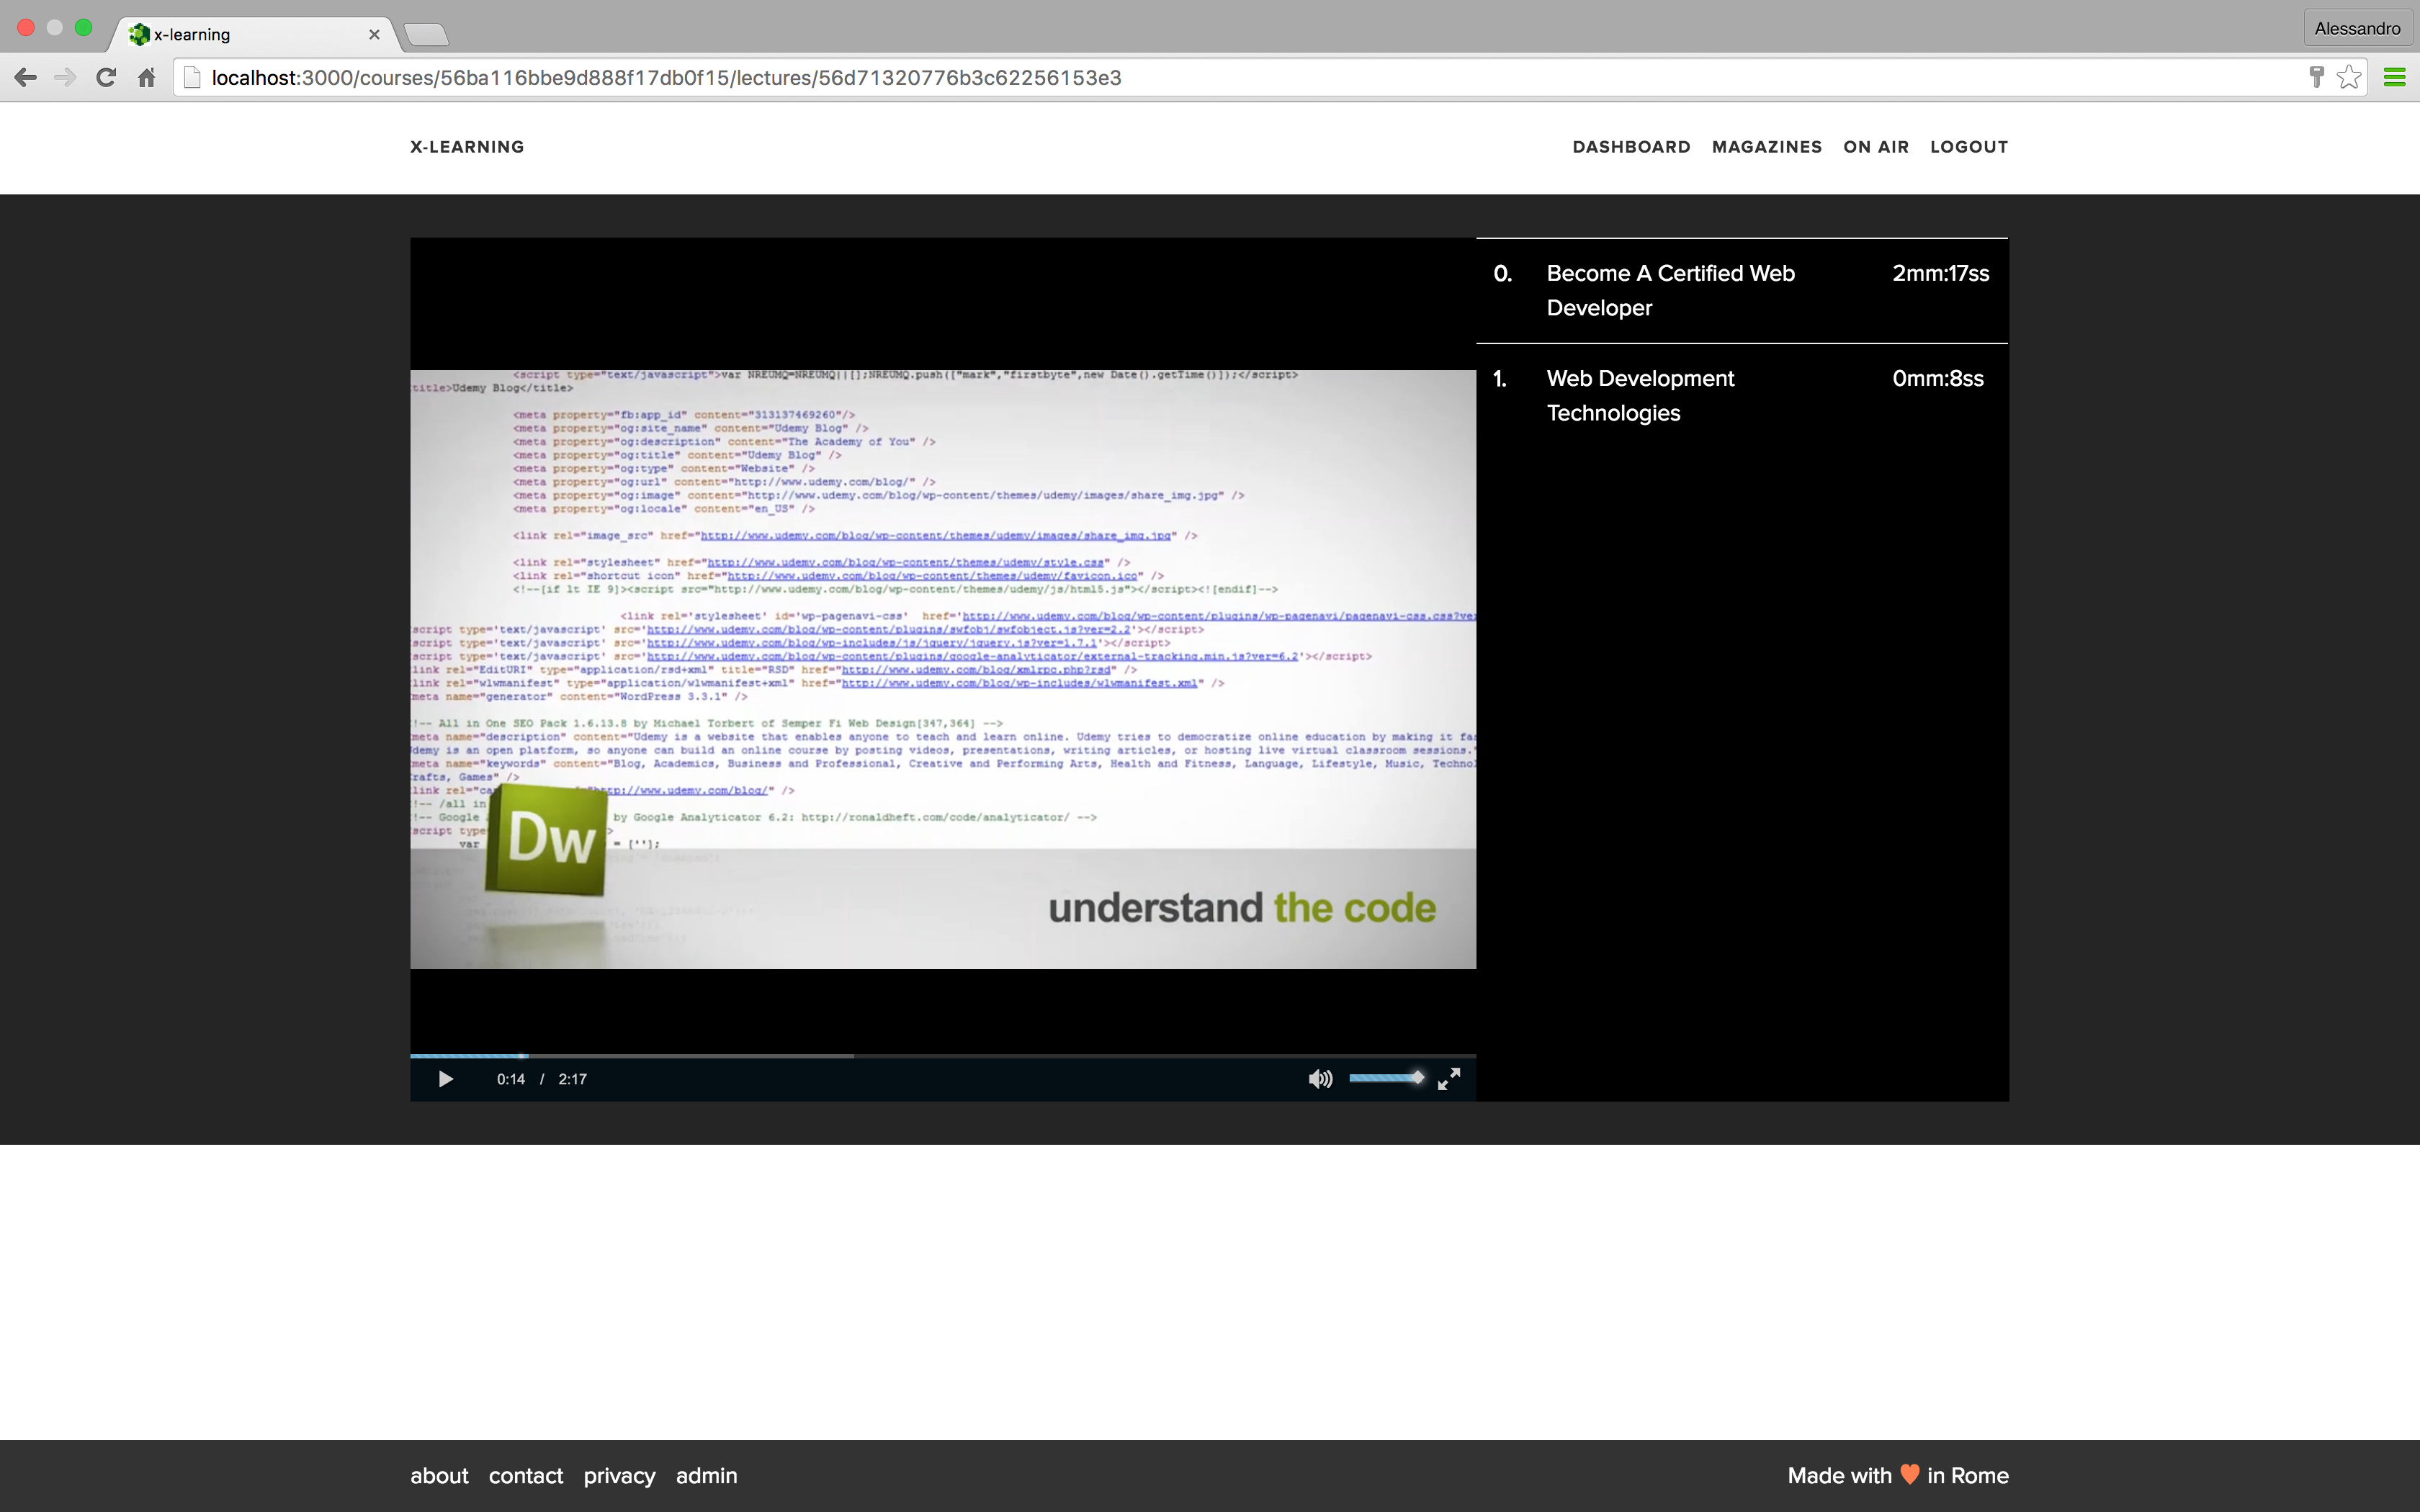
\includegraphics[width=1.0\linewidth]{images/chapter5/page-lecture-deck.png}\hfill
 \caption[Video player]{Video player}
 \label{fig:fourV}
\end{figure}
